\documentclass[12pt]{amsart}

\usepackage[
	paperheight=11in,
	paperwidth=8.5in,
	inner=0.4in,
	textheight=10.2in,
	textwidth=7.5in,
	% marginparwidth=120pt,
	% marginparsep=32pt,
	% bottom=1.4in,
	% left=0.5in,
	% right=0.5in,
	% footskip=1.0in
]{geometry}
\geometry{letterpaper}

\usepackage{array}
\usepackage{amssymb}
\usepackage{asymptote}
\usepackage{amsmath}
\usepackage{amsfonts}
\usepackage{animate}
\usepackage{arrayjobx}
\usepackage{arydshln}
\usepackage{bookman}
\usepackage{color}
\usepackage{cancel}
\usepackage{calculator}
\usepackage{collcell}
\usepackage{epstopdf}
\usepackage{enumerate}
\usepackage{epsfig}
\usepackage[english]{babel}
\usepackage{etoolbox}
\usepackage{fancyhdr}
\usepackage{fancybox}
\usepackage[nomessages]{fp}
\usepackage{graphics}
\usepackage{graphicx}
\usepackage{ifthen}
\usepackage{ifmtarg}
\usepackage[latin1]{inputenc}
\usepackage{latexsym}
\usepackage{multirow}
\usepackage{multicol}
\usepackage{multimedia}
\usepackage{mathbbol}
\usepackage{mathtools}
\usepackage{multido}
\usepackage{palatino}
\usepackage{polynom}
\usepackage{pxfonts}
\usepackage{pifont}
\usepackage{pgffor}
\usepackage{pdfpages}
\usepackage[parfill]{parskip}
\usepackage{soul}
\usepackage{tikz}
\usetikzlibrary{arrows,shapes,trees,shapes.geometric,calc}
\usepackage{txfonts}
\usepackage{tcolorbox}
\usepackage{wasysym}
\usepackage{wrapfig}
\usepackage{xcolor}
\usepackage{xmpmulti}
\usepackage{xparse}
\usepackage{xstring}
\usepackage{mathrsfs}
\newcommand{\LAP}[1]{\mathscr{L}\{#1\}}

\renewcommand{\headrulewidth}{0pt} % remove lines as well

\numberwithin{equation}{section}

\DeclareGraphicsRule{.tif}{png}{.png}{`convert #1 `dirname #1`/`basename #1 .tif`.png}

\newcounter{ProbNum}
\setcounter{ProbNum}{0}
\def\NEWPROB{\stepcounter{ProbNum} {\noindent \arabic{ProbNum}. \,\,}}

\begin{document}

	\pagestyle{empty}

	\hrule
	\begin{center}
		\begin{tabular}{p{6.8in}}
			\multicolumn{1}{c}{\sc Differential Equations} \\
			\multicolumn{1}{c}{\sc Laplace Transforms}
		\end{tabular}
	\end{center}
	\medskip
	\hrule

	\medskip

	\underline{Laplace Transform}

	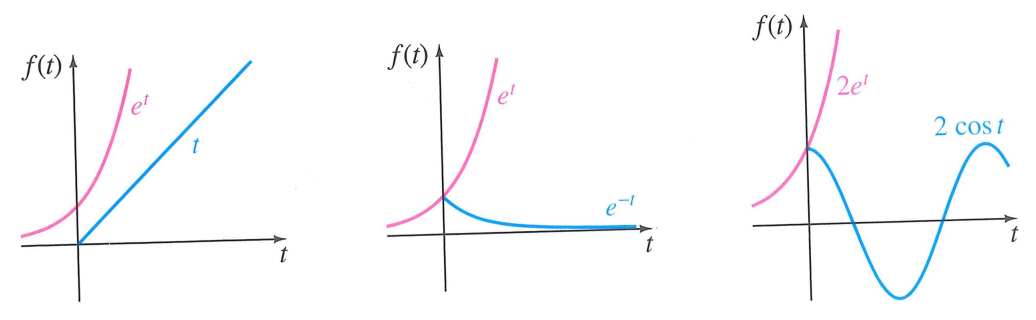
\includegraphics[scale=0.8]{exponential-growth-figs.png}

	\NEWPROB Compute the following limits:

	\begin{enumerate}
		\item \(\displaystyle \lim_{t\to\infty} e^{t} = \)
		\vfill
		\item \(\displaystyle \lim_{t\to\infty} te^{t} = \)
		\vfill
		\item \(\displaystyle \lim_{t\to\infty} e^{-t} = \)
		\vfill
		\item \(\displaystyle \lim_{t\to\infty} te^{-t} = \)
		\vfill
		\item \(\displaystyle \lim_{t\to\infty} e^{-t}\cos(t) = \)
		\vfill
		\item \(\displaystyle \text{if}\ s > 0\ \text{then}\quad\lim_{t\to\infty} te^{st} = \)
		\vfill
		\item \(\displaystyle \text{if}\ s = 0\ \text{then}\quad\lim_{t\to\infty} te^{st} = \)
		\vfill
		\item \(\displaystyle \text{if}\ s < 0\ \text{then}\quad\lim_{t\to\infty} te^{st} = \)
		\vfill
	\end{enumerate}

	\newpage
	\thispagestyle{empty}

	\noindent The Laplace Transform of function $f(t)$ is a new function $F(s)$ defined by:
	\[ 
		F(s) = \LAP{f(t)} = \int_0^{\infty}e^{-st}f(t) dt,
	\]
	provided this integral is finite (converges).
		
	\NEWPROB Use the definition of Laplace Transform (above) to find the Laplace Transform of $h(t) = 7t.$  
	Include appropriate restrictions on $s$ to guarantee the convergence of the integral.

	\newpage
	\thispagestyle{empty}

	\NEWPROB Use the definition of Laplace Transform (above) to find the Laplace Transform of  the function
	\[
		d(t) = 
		\left\{ 
			\begin{array}{ll}
				0,	& t<0\\
				7,	& 0 \le t < 3\\
				0,	& t \ge 3\\
			\end{array}
		\right.
	\]
	
	Include appropriate restrictions on $s$ to guarantee the convergence of the integral.

	\newpage
	\thispagestyle{empty}

	\NEWPROB Show that the Laplace Transform has the following 2 properties:

	\begin{enumerate}
		\item  $\displaystyle \LAP{f(t)+g(t)} = \LAP{f(t)}+\LAP{g(t)}$
		\vspace{10.2cm}
		\item  $\displaystyle \LAP{A f(t)} = A \LAP{f(t)}\quad $($A$ is constant)
	\end{enumerate}

	\newpage
	\thispagestyle{empty}

	\NEWPROB Determine the Laplace transform of each function. Use the table given in class.
	%-------NUM LIST---------
	\begin{itemize}
		\item  $f(t) = e^{-2t}$
		\vspace{5.2cm}
		\item  $g(t) = t^3 $
		\vspace{5.2cm}
		\item  $h(t) = e^{2t} - \sin(5t)$
		\vspace{5.2cm}
		\item  $q(t) = 8t + 4 - \cos(6t)$
		\vspace{5.2cm}
	\end{itemize}

\end{document}